\section{PC mjukvara}
PC-mjukvaran har som uppgift att låta användaren kommunicera med roboten via ett
enkelt gränssnitt. Via PC-mjukvaran kan användaren få intressant information
från robotens olika moduler, t.ex avstånd till väggar eller vilket styrkommando
som nu utförs. PC-mjukvaran kommunicerar med roboten via blåtand.

\subsection{Implementation}

Mjukvaran är skriven i programspråket C och använder utöver Cs standardbibliotek
även gränssnittet BlueZ för att kommunicera via blåtand, biblioteket SDL för att
generera kommandon till roboten via tangentbordet samt NCurses för att
åskådliggöra information i terminalen på ett trevligt och överskådligt sätt..

Mjukvaran består av två huvuddelar, input\_control samt send\_receive. input\_control
hanterar knapptryckningar från användaren och genererar instruktioner att skicka
till roboten, intruktionen placeras sedan i en enkel databas (instr\_db).
send\_receive i sin tur läser in instruktionen från databasen och om användaren
har genererat en ny instruktion kommer denna skickas till roboten via blåtand
(instruktioner som redan skcikat till roboten kommer alltså inte att skickas
 igen), ifall instruktionen innehåller information om önskad hastighet på
roboten eller trimnivåer på motorerna så kommer detta också visas på skärmen.
När instruktionen skickats till roboten kommer send\_receive invänta 2 databyte
från roboten (vilket kan vara sensorinfo, specialkommando el. dyl.) som sedan
kommer åskådligjöras på skärmen.

\subsubsection{Gränssnittet}

\begin{figure}[H]
        \centering
        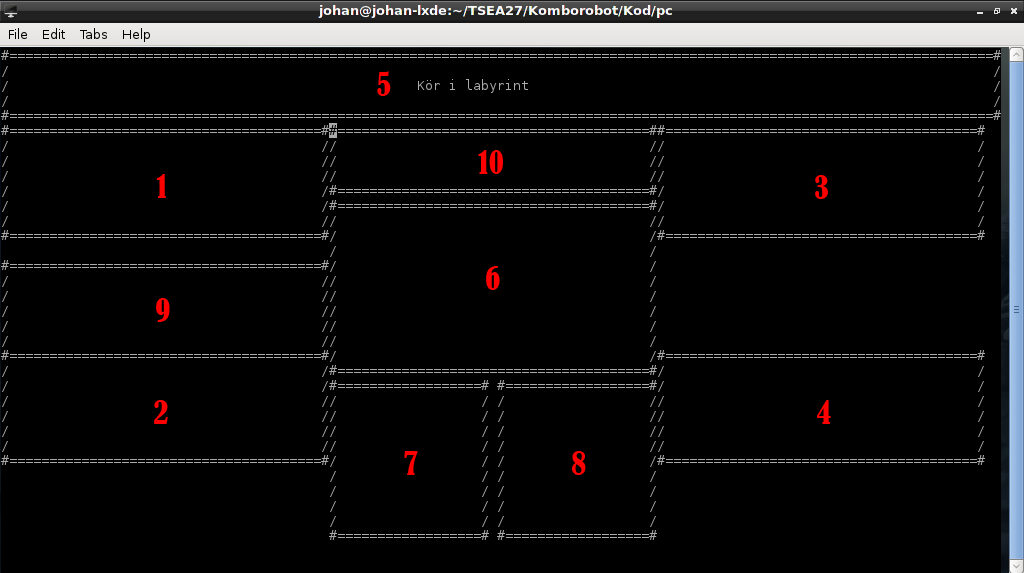
\includegraphics[scale=0.5]{bilder/granssnitt.png}
        \caption{Användargränssnittet för send\_receive}
        \label{fig:sendrec}
\end{figure}
\begin{enumerate}
\item Avståndssensor, vänster fram på Komborobot.
\item Avståndssensor, vänster bak på Komborobot.
\item Avståndssensor, höger fram på Komborobot.
\item Avståndssensor, höger bak på Komborobot.
\item Labyrintläge, linjeföljarläge eller fjärrstyrt läge.
\item Senast skickad hastighet.
\item Trimnivå vänster motor.
\item Trimnivå höger motor.
\item Felaktigt kommando skickat till styrenheten.
\item Senast utförda specialkommandon.

\begin{figure}[H]
        \centering
        
\includegraphics[scale=0.5]{bilder/input_control.png}
        \caption{Användargränssnittet för input\_control}
        \label{fig:inputcont}
\end{figure}

\item input\_control.

\end{enumerate}
\subsection{Användande} 

För att börja använda roboten startar man först programmet input\_control, detta
initierar databasen instr\_db och ger användaren möjlighet att skapa
styrkommandon åt roboten med hjälp av tangentbordstryckningar. Sedan startar man
programmet send\_receive som ansluter till roboten via blåtand och börjar skicka
samt ta emot data från roboten.

Då roboten befinner sig i fjärrstyrt läge används följande tangentbindningar för
att generera styrkommandon: 
\begin{itemize}
\item w - Kör framåt
\item s - Kör bakåt
\item a - rotera vänster
\item d - rotera höger
\item q - vänstersväng (mjuk kurva)
\item e - högersväng (mjuk kurva)
\item mellanslag - stanna roboten
\item pil upp - öka hastigheten, ingen effekt tills man skickar ett kommando somutnyttjar hastigheten
\item pil ner - sänk hastigheten, ingen effekt tills man skickar ett kommando som utnyttjar hastigheten.
\item pil höger - trim höger, öka effekten på höger motor en aning (små steg, användbart för finjustering)
\item pil vänster - trim vänster, öka effekten på vänster motor en aning (små steg, användbart för finjustering)
\item o - nollställ trim
\item u - öka linjesensorklibreringskonstanten 
\item i - minska linjesensorkalibreringskonstanten
\item c - kalibrera linjesensorerna med värdet sparat i
linjesensorkalibreringskonstanten
\item esc - avsluta input control
\end{itemize}

Värdet på linjesensorkalibreringskonstanten anges inte exakt, däremot så anger
färgen på input\_control ett ungeförligt värde.

För att avsluta send\_receive används <ctr + c> vilket kommer återställa
terminalen åt användaren.
